\documentclass[a4paper,10pt]{article}
\usepackage[utf8]{inputenc}
\usepackage[utf8]{inputenc}
\usepackage[default,osfigures,scale=0.95]{opensans}\usepackage{graphicx}
\usepackage{graphicx}
\usepackage{epsfig}
\usepackage{german}
\usepackage{url}
\usepackage{fancyhdr}
\hyphenation{me-cha-nik}

\pagestyle{fancy}
\fancyhf{}
\fancyhead[L]{
	
\includegraphics[scale=0.1]{./figures/logo.png}
}
%\fancyhead[C]{}
%\fancyfoot[L]{Erstellt am: \today}
\fancyfoot[R]{\thepage}
\setlength{\headheight}{20pt}
\setlength{\parindent}{0pt}

\begin{document}

\vspace*{1cm}

{\bfseries \large Layoutvorschlag \\[1mm]
\normalfont Autor: Elizaveta Ragozina}					%Autor sollte immer angegeben werden

\vspace{1cm}

\begin{abstract}
	Dieses Dokument umfasst Entwürfe einiger Orte, an denen das Spiel abläuft. Erste Eindrücke eines Minispiels und des Smartphones sind ebenfalls zu sehen.
\end{abstract}

\newpage

\begin{figure}
	\centering
	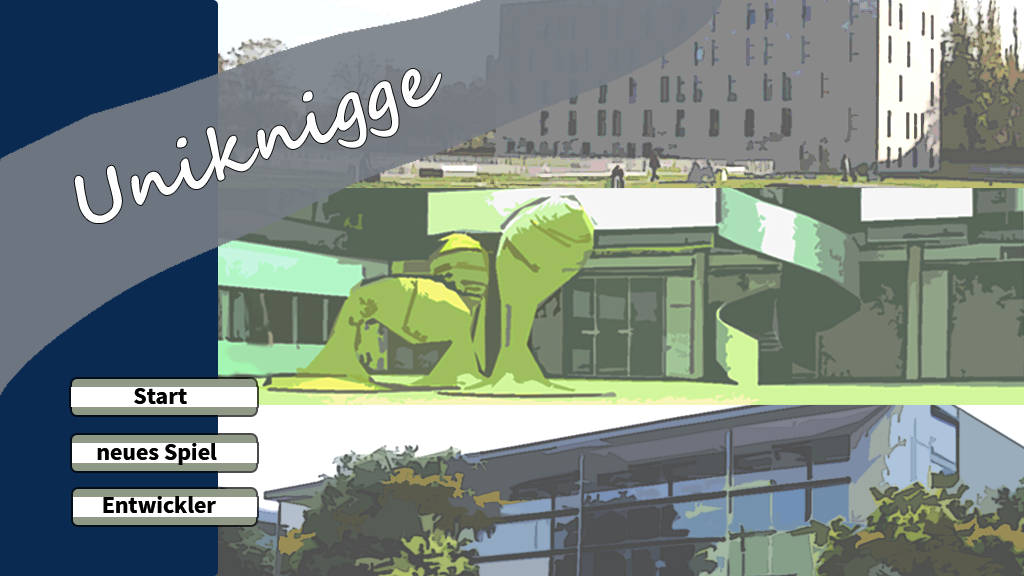
\includegraphics[width=\textwidth]{./figures/mainmenu.png}
	\caption{Das Hauptmenü}
\end{figure}

\begin{figure}
	\centering
	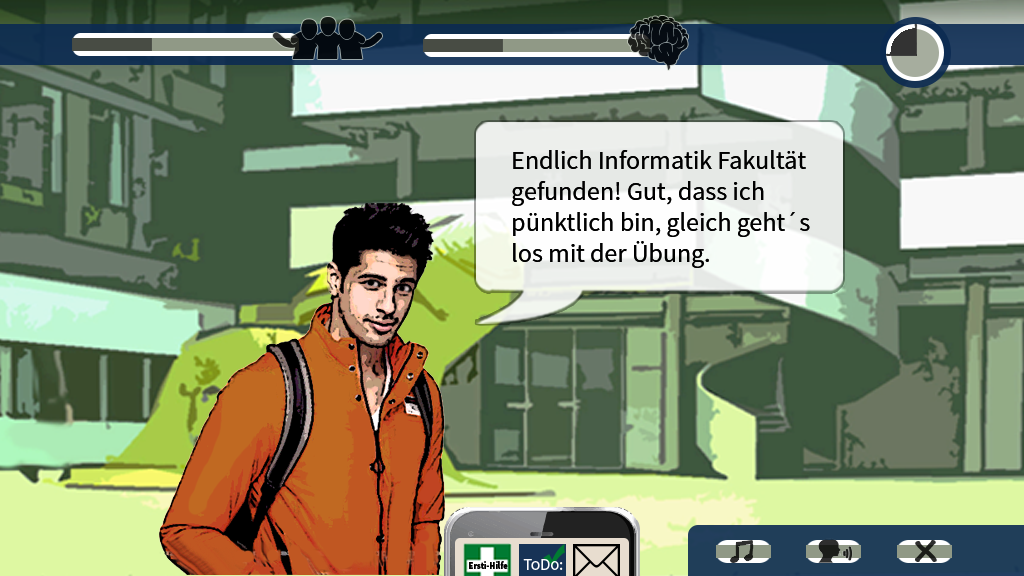
\includegraphics[width=\textwidth]{./figures/apb.png}
	\caption{Protagonist im Andreas-Pfitzmann-Bau}
\end{figure}

\begin{figure}
	\centering
	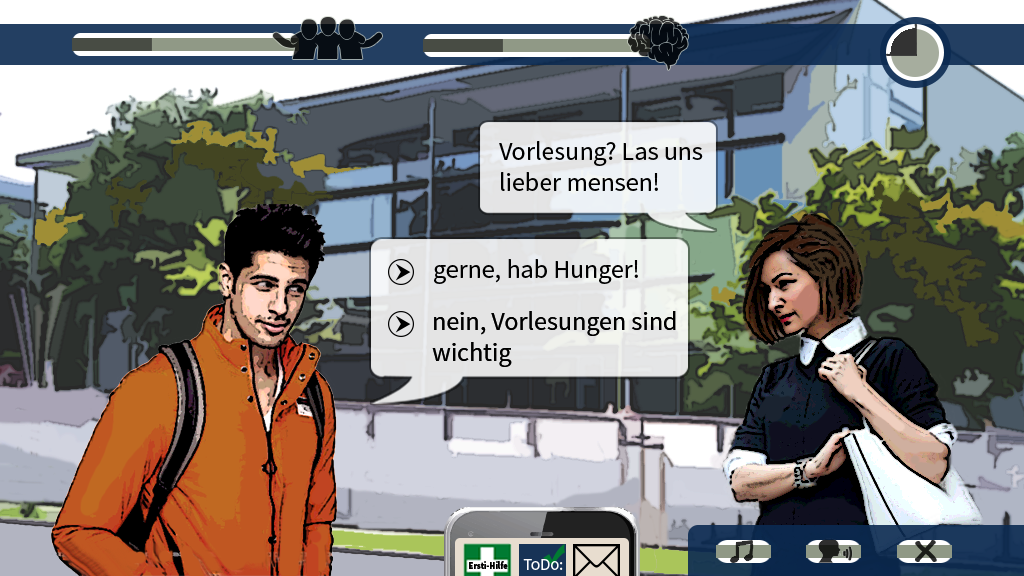
\includegraphics[width=\textwidth]{./figures/hsz.png}
	\caption{Protagonist mit Kommilitonin vor dem Hörsaalzentrum}
\end{figure}

\begin{figure}
	\centering
	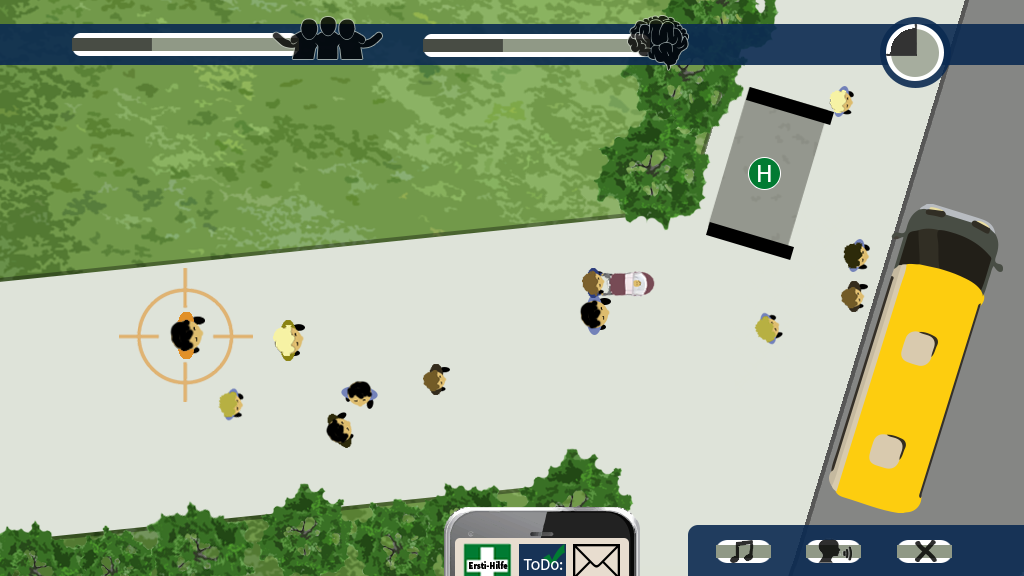
\includegraphics[width=\textwidth]{./figures/busspiel.png}
	\caption{Entwurf eines Minigames}
\end{figure}

\begin{figure}
	\centering
	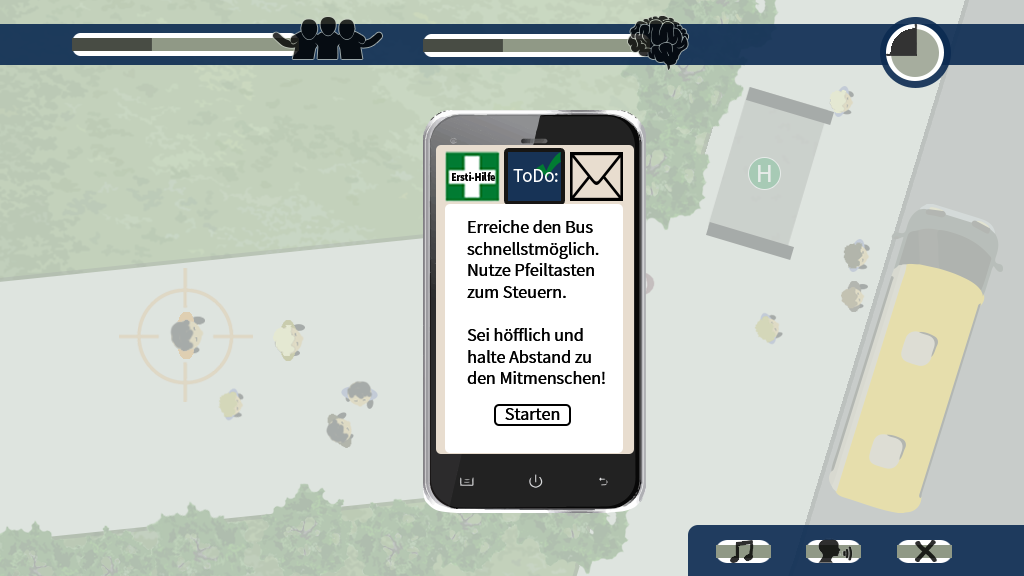
\includegraphics[width=\textwidth]{./figures/smartphone.png}
	\caption{Smartphone des Protagonisten (Hilfe für den Lernenden)}
\end{figure}

\end{document}